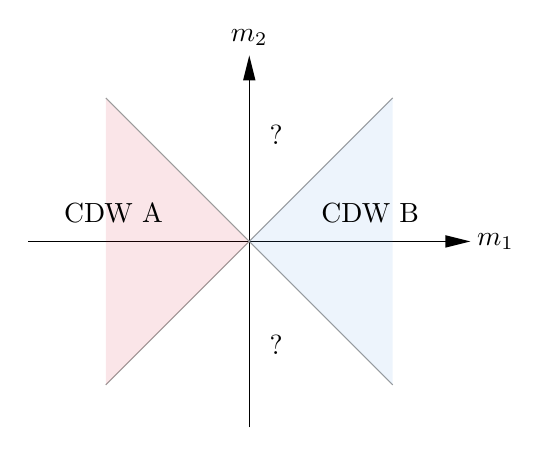
\begin{tikzpicture}[x=0.75pt,y=0.75pt,yscale=-1,xscale=1]
    %uncomment if require: \path (0,300); %set diagram left start at 0, and has height of 300
    
    %Straight Lines [id:da4723682080175666] 
    \draw    (100,115) -- (311,115) ;
    \draw [shift={(313,115)}, rotate = 180] [fill={rgb, 255:red, 0; green, 0; blue, 0 }  ][line width=0.08]  [draw opacity=0] (12,-3) -- (0,0) -- (12,3) -- cycle    ;
    %Straight Lines [id:da8644421157617888] 
    \draw    (206.5,204.58) -- (206.5,27.42) ;
    \draw [shift={(206.5,25.42)}, rotate = 90] [fill={rgb, 255:red, 0; green, 0; blue, 0 }  ][line width=0.08]  [draw opacity=0] (12,-3) -- (0,0) -- (12,3) -- cycle    ;
    %Straight Lines [id:da8934475925664409] 
    \draw [color={rgb, 255:red, 155; green, 155; blue, 155 }  ,draw opacity=1 ]   (137.38,184.12) -- (275.62,45.88) ;
    %Shape: Polygon [id:ds582430351802862] 
    \draw  [draw opacity=0][fill={rgb, 255:red, 208; green, 2; blue, 27 }  ,fill opacity=0.1 ] (137.38,184.12) -- (137.38,45.88) -- (206.5,115) -- cycle ;
    %Straight Lines [id:da12297920958446729] 
    \draw [color={rgb, 255:red, 155; green, 155; blue, 155 }  ,draw opacity=1 ]   (275.62,184.12) -- (137.38,45.88) ;
    %Shape: Polygon [id:ds5009441910042658] 
    \draw  [draw opacity=0][fill={rgb, 255:red, 74; green, 144; blue, 226 }  ,fill opacity=0.1 ] (275.62,184.12) -- (275.62,45.88) -- (206.5,115) -- cycle ;
    
    % Text Node
    \draw (315,115) node [anchor=west] [inner sep=0.75pt]    {$m_{1}$};
    % Text Node
    \draw (206.5,22.02) node [anchor=south] [inner sep=0.75pt]    {$m_{2}$};
    % Text Node
    \draw (240,95.5) node [anchor=north west][inner sep=0.75pt]   [align=left] {CDW B};
    % Text Node
    \draw (116,95.5) node [anchor=north west][inner sep=0.75pt]   [align=left] {CDW A};
    % Text Node
    \draw (215,58) node [anchor=north west][inner sep=0.75pt]   [align=left] {?};
    % Text Node
    \draw (215,159) node [anchor=north west][inner sep=0.75pt]   [align=left] {?};
    
    
    \end{tikzpicture}
    